\documentclass{sigchi-ext}
% Please be sure that you have the dependencies (i.e., additional
% LaTeX packages) to compile this example.
\usepackage[T1]{fontenc}
\usepackage{textcomp}
\usepackage[scaled=.92]{helvet} % for proper fonts
\usepackage{graphicx} % for EPS use the graphics package instead
\usepackage{balance}  % for useful for balancing the last columns
\usepackage{booktabs} % for pretty table rules
\usepackage{ccicons}  % for Creative Commons citation icons
\usepackage{ragged2e} % for tighter hyphenation

% Some optional stuff you might like/need.
% \usepackage{marginnote} 
% \usepackage[shortlabels]{enumitem}
% \usepackage{paralist}
% \usepackage[utf8]{inputenc} % for a UTF8 editor only

%% EXAMPLE BEGIN -- HOW TO OVERRIDE THE DEFAULT COPYRIGHT STRIP --
% \copyrightinfo{Permission to make digital or hard copies of all or
% part of this work for personal or classroom use is granted without
% fee provided that copies are not made or distributed for profit or
% commercial advantage and that copies bear this notice and the full
% citation on the first page. Copyrights for components of this work
% owned by others than ACM must be honored. Abstracting with credit is
% permitted. To copy otherwise, or republish, to post on servers or to
% redistribute to lists, requires prior specific permission and/or a
% fee. Request permissions from permissions@acm.org.\\
% {\emph{CHI'14}}, April 26--May 1, 2014, Toronto, Canada. \\
% Copyright \copyright~2014 ACM ISBN/14/04...\$15.00. \\
% DOI string from ACM form confirmation}
%% EXAMPLE END

% Paper metadata (use plain text, for PDF inclusion and later
% re-using, if desired).  Use \emtpyauthor when submitting for review
% so you remain anonymous.
\def\plaintitle{PrePre: Presence and Pressure Sensing} \def\plainauthor{First Author, Second Author, Third Author,
  Fourth Author, Fifth Author, Sixth Author}
\def\emptyauthor{}
\def\plainkeywords{Authors' choice; of terms; separated; by
  semicolons; include commas, within terms only; required.}
\def\plaingeneralterms{Documentation, Standardization}

\title{PrePre: Presence and Pressure Sensing}

\numberofauthors{6}
% Notice how author names are alternately typesetted to appear ordered
% in 2-column format; i.e., the first 4 autors on the first column and
% the other 4 auhors on the second column. Actually, it's up to you to
% strictly adhere to this author notation.
\author{%
  \alignauthor{%
    \textbf{Troy Nachtigall}\\
    \affaddr{Eindhoven Univsersity of Technology} \\
    \affaddr{Eindhoven,  5400MB, NL} \\
    \email{t.r.nachtigall@tue.nl} }
    \alignauthor{%
    \textbf{A.M.J.M. Schoonen}\\
    \affaddr{Eindhoven, The Netherlands}\\
    \email{admar@familieschoonen.nl} } 
    }

\begin{marginfigure}
\begin{minipage}{\marginparwidth}
\centering
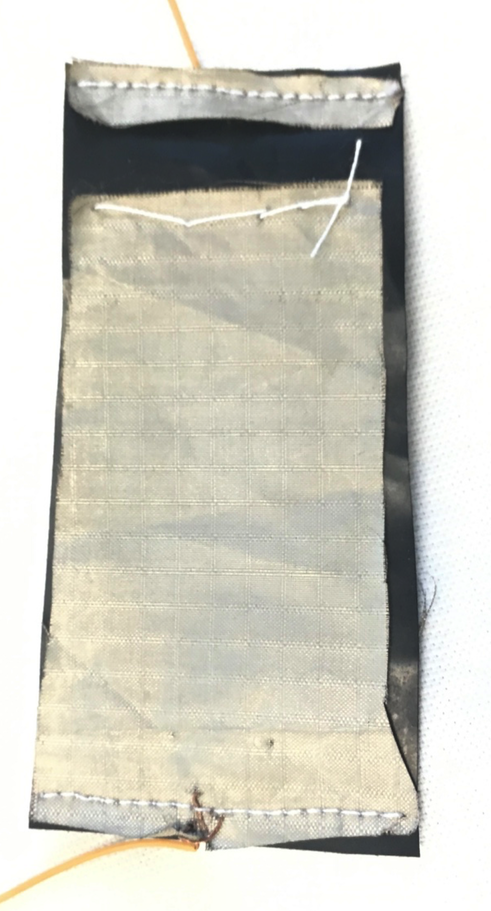
\includegraphics[width=0.9\columnwidth]{figures/sensor}
 \caption{PrePre sensor prototype.}~\label{fig:sensor}
\end{minipage}
\end{marginfigure}

% Make sure hyperref comes last of your loaded packages, to give it a
% fighting chance of not being over-written, since its job is to
% redefine many LaTeX commands.
\definecolor{linkColor}{RGB}{6,125,233}
\hypersetup{%
  pdftitle={\plaintitle},
%  pdfauthor={\plainauthor},
  pdfauthor={\emptyauthor},
  pdfkeywords={\plainkeywords},
  bookmarksnumbered,
  pdfstartview={FitH},
  colorlinks,
  citecolor=black,
  filecolor=black,
  linkcolor=black,
  urlcolor=linkColor,
  breaklinks=true,
}

% \reversemarginpar%

\begin{document}

\maketitle

% Uncomment to disable hyphenation (not recommended)
% https://twitter.com/anjirokhan/status/546046683331973120
\RaggedRight{} 

% Do not change the page size or page settings.
\begin{abstract}
  Designing with properties such as touch and  distance 
  sensing in electronics and digital control enables new dimensions within fashion and design, and a range of new possibilities for sensing, tactility and functionality. Resistive pressure sensing and capacitive presence sensing are not new in wearable technology. However, there is still limited insight into the potential of soft materials capable of performing multiple functions at the same time. Adding multiple functionalities is fundamental to the exploitation of new e-textile properties. Development of multifunctional textiles may provide greater use possibilities for e-textiles where separate components for each sensor were required. This submission to the ISWC Fiber arts design competition demonstrates  a method to add presence sensing to pressure sensors, allowing to detect the presence of humans before they touch the pressure sensor.  This allows for novel interfaces that guide users even before they deliberately use and interact with the object. In principle, the method only requires a software modification so there are no
  additional costs for materials and the feature could be made available to
  existing products with a software update.   This textile is a prime example the design research into wearable technology of Troy Nachtigall coming together with the particular capacitive engineering expertise of Admar Schoonen. Together they create a new smart textile with multi functionalities that sense presence and pressure.  
\end{abstract} 


    
\keywords{\plainkeywords}
\category{H.5.2.Information Interfaces and Presentation, 
  I.4.8 Sensor Fusion}
\keywords{Sensor; Sensing; Presence; Pressure; Capacitive; Resistive; Textile; E-textile
}

\begin{marginfigure}
\begin{minipage}{\marginparwidth}
\centering
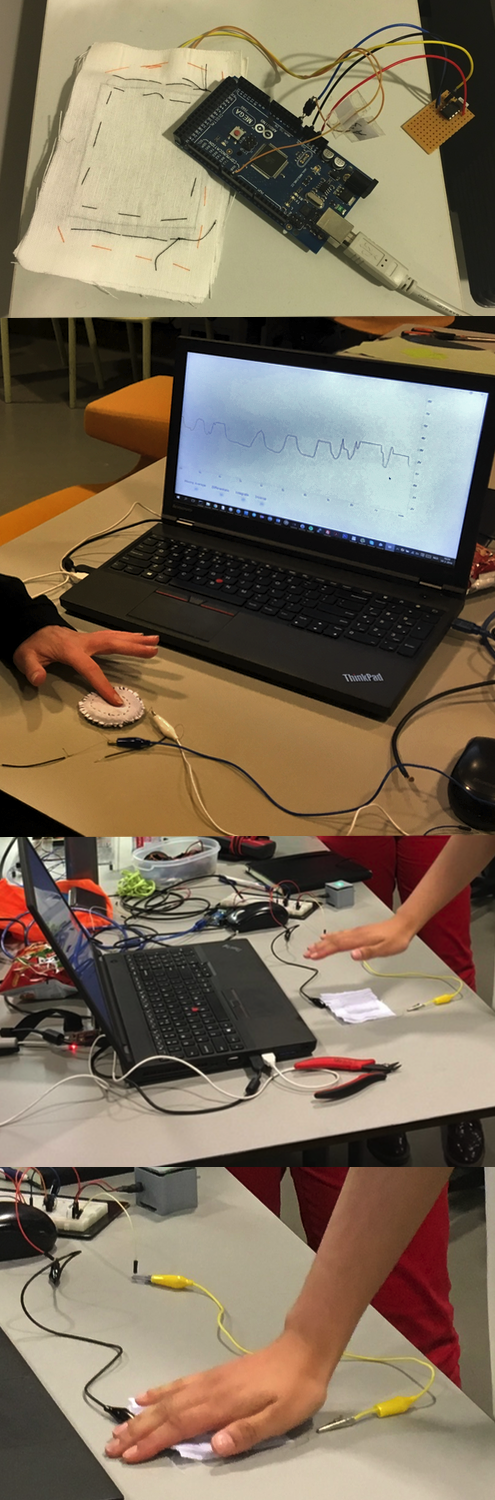
\includegraphics[width=0.9\columnwidth]{figures/workshop}
 \caption{PrePre workshop testing materials and configurations at the TU/e E-Lab.}~\label{fig:workshop}
\end{minipage}
\end{marginfigure}

\section{Introduction}
Troy Nachtigall is a Wearable Technology expert currently exploring programming materials as a Marie Sladowska Curie research fellow in the ArcInTexETN Horizon 2020 project where he explores the relationship of adaptive and responsive wearables between the scales of the individual, the room and architecture. Engineer Admar Schoonen is an expert in capacitive technologies with many projects in capacitive touch sensing.  He is a member of the TU/Eindhoven Industrial Design /dSearch labs exploring design research from an engineering perspective.  PrePre presents a design collaboration between Troy and Admar to create an e-textile and supporting code to sense pressure and  presence on as many as four sensors simultaneously.  This collaborative process was selected for a pair of workshops at the Ultra Personalized Smart Textiles (UPST) project at the University of Technology at Eindhoven in part as an ambassador action of the ArcInTexETN Horizon 2020 project (www.ArcInTexETN.eu). These workshops explored iterations of touch and presence technologies with interaction designers where new frontiers of sensing and actuating were explored.  
\section{Design}
The capability of sensing not only when someone is pressing against a textile, but when they are approaching the textile adds new dimensions to interaction and the design of those interactions.  While the sensor can be made with conductive, resistive and insulating materials, the sensor is intended for 'on the body' and 'near the body' uses where softness and tactility are highly valued and often product features. 
\subsection{Design Concept}
Touch is important in interaction, but vicinity is often revealing of behavior and motivations.  Not only can vicinity detect hesitation or reluctance in touching, but vicinity can also reveal choosing not to touch. This becomes very interesting when deployed in a garment worn on the body. In the process of iterative design development this 'on the body' aspect became increasingly interesting. The decision to add a shielding layer to the sensor allows for the use of the PrePre on the body which is difficult as the capacitative sensor typically sees both sides. After several workshops with designers of the Ultra Personalized Smart Textiles research group, Figure \ref{fig:workshop}, not only were choices of textiles perfected, but the technique of capacitative sensing was tailored as well. At the same time the aesthetic qualities were considered as the PrePre is intended for fashion. The PrePre sample is novel in its dual nature of sensing pressure and presence at the same time. Since it requires no extra hardware or fabric layers, garments can be thinner, more flexible and breathable as well as lower cost and with lower impact on environment.
\subsection{Textiles}
A low density ESD Foam\footnote{\url{http://nl.farnell.com/multicomp/039-0050/low-density-foam-305x305x6mm/dp/1687866}} was chosen for the resistive layer for its spacer fabric qualities.  The low density aspect causes the foam to lift back up quickly after the touch is released which helps mitigate hysteresis. A highly conductive silver coated e-textile knit Dorlastan was chosen for the electrode layers due to its soft yet highly conductive feature. The stretch version was chosen to once again aid in resiliency which helps the sensor return to it's original state when released.  An hydrophobic polyester was chosen for the insulating layers to protect the conductive layers and prevent influence from humidity.  A conductive ripstop nylon was selected for the shielding layer for its conductive conformity. An overview of the stackup of the different materials is shown in Figure \ref{fig:stackup}.

% \begin{marginfigure}
% \begin{minipage}{\marginparwidth}
% \centering
% 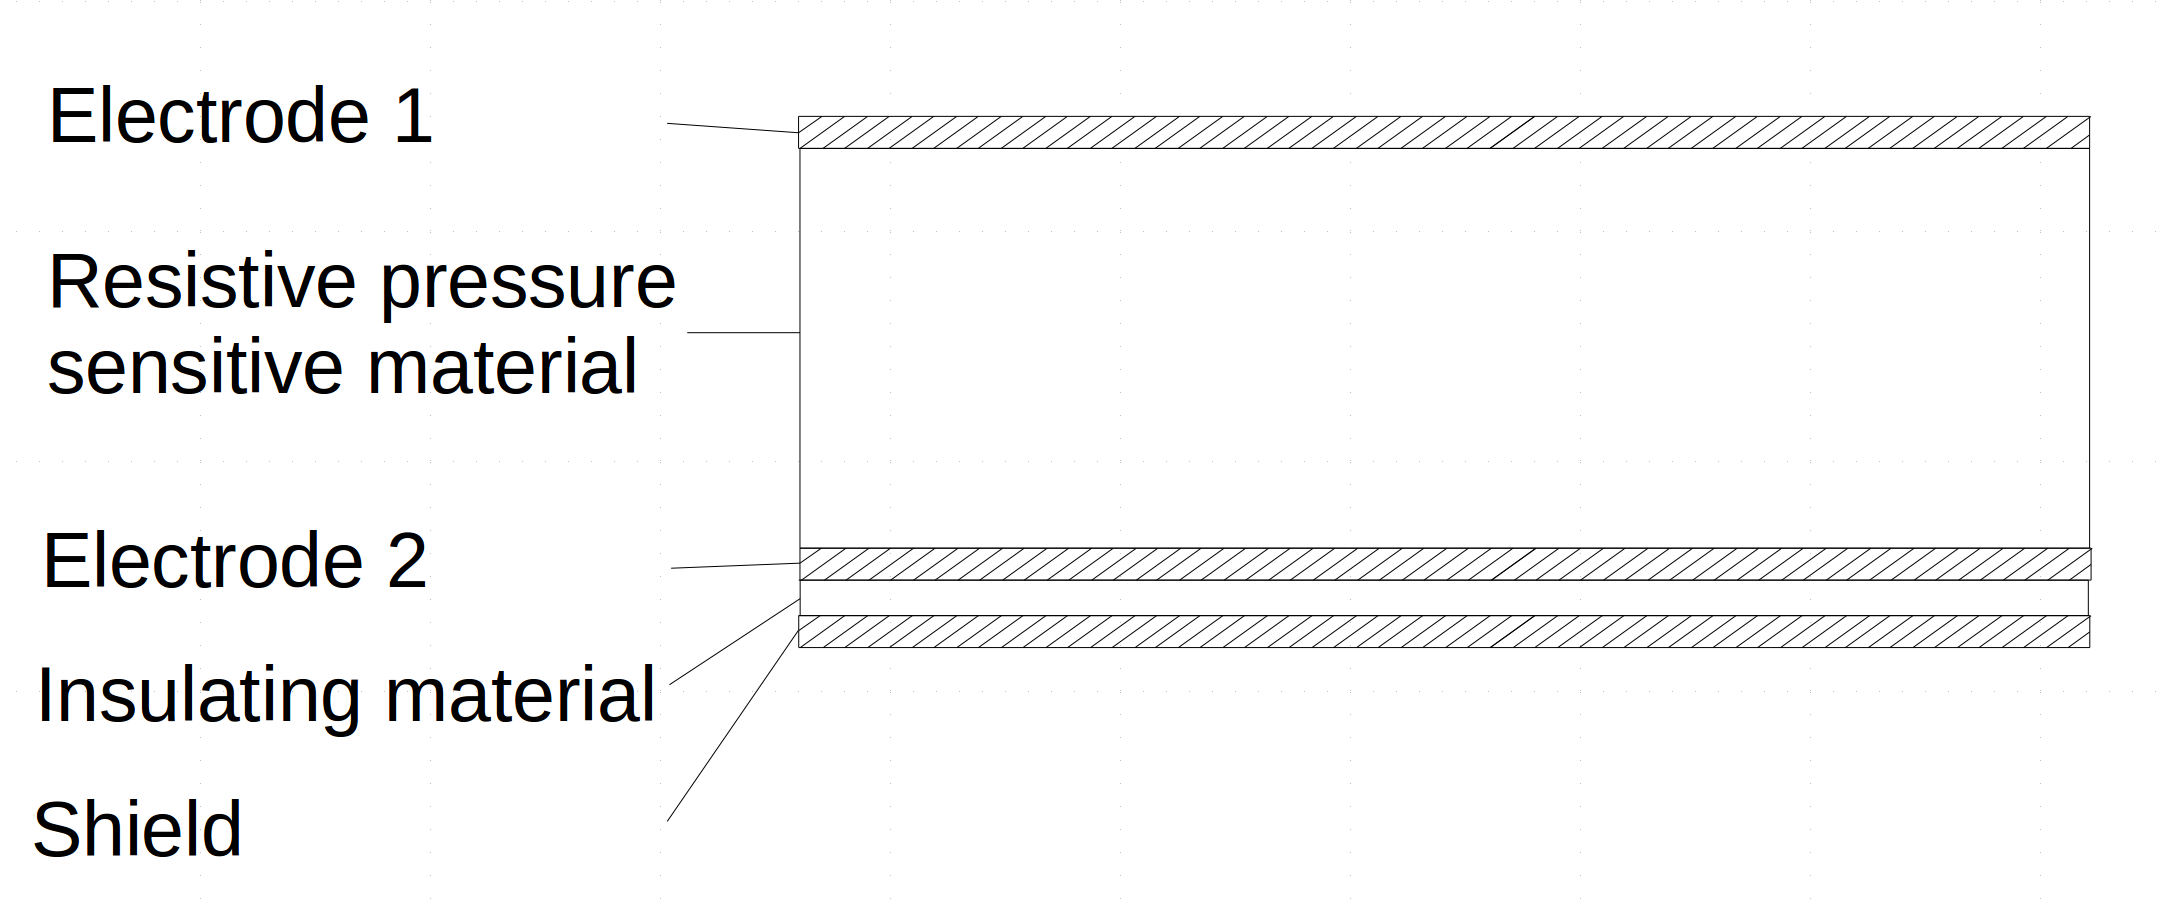
\includegraphics[width=0.9\columnwidth]{figures/stackup}
% \caption{Stackup for pressure and presence sensor with
% shield}~\label{fig:stackup}
% \end{minipage}
% \end{marginfigure}

\begin{figure}[!htbp]
\centering
  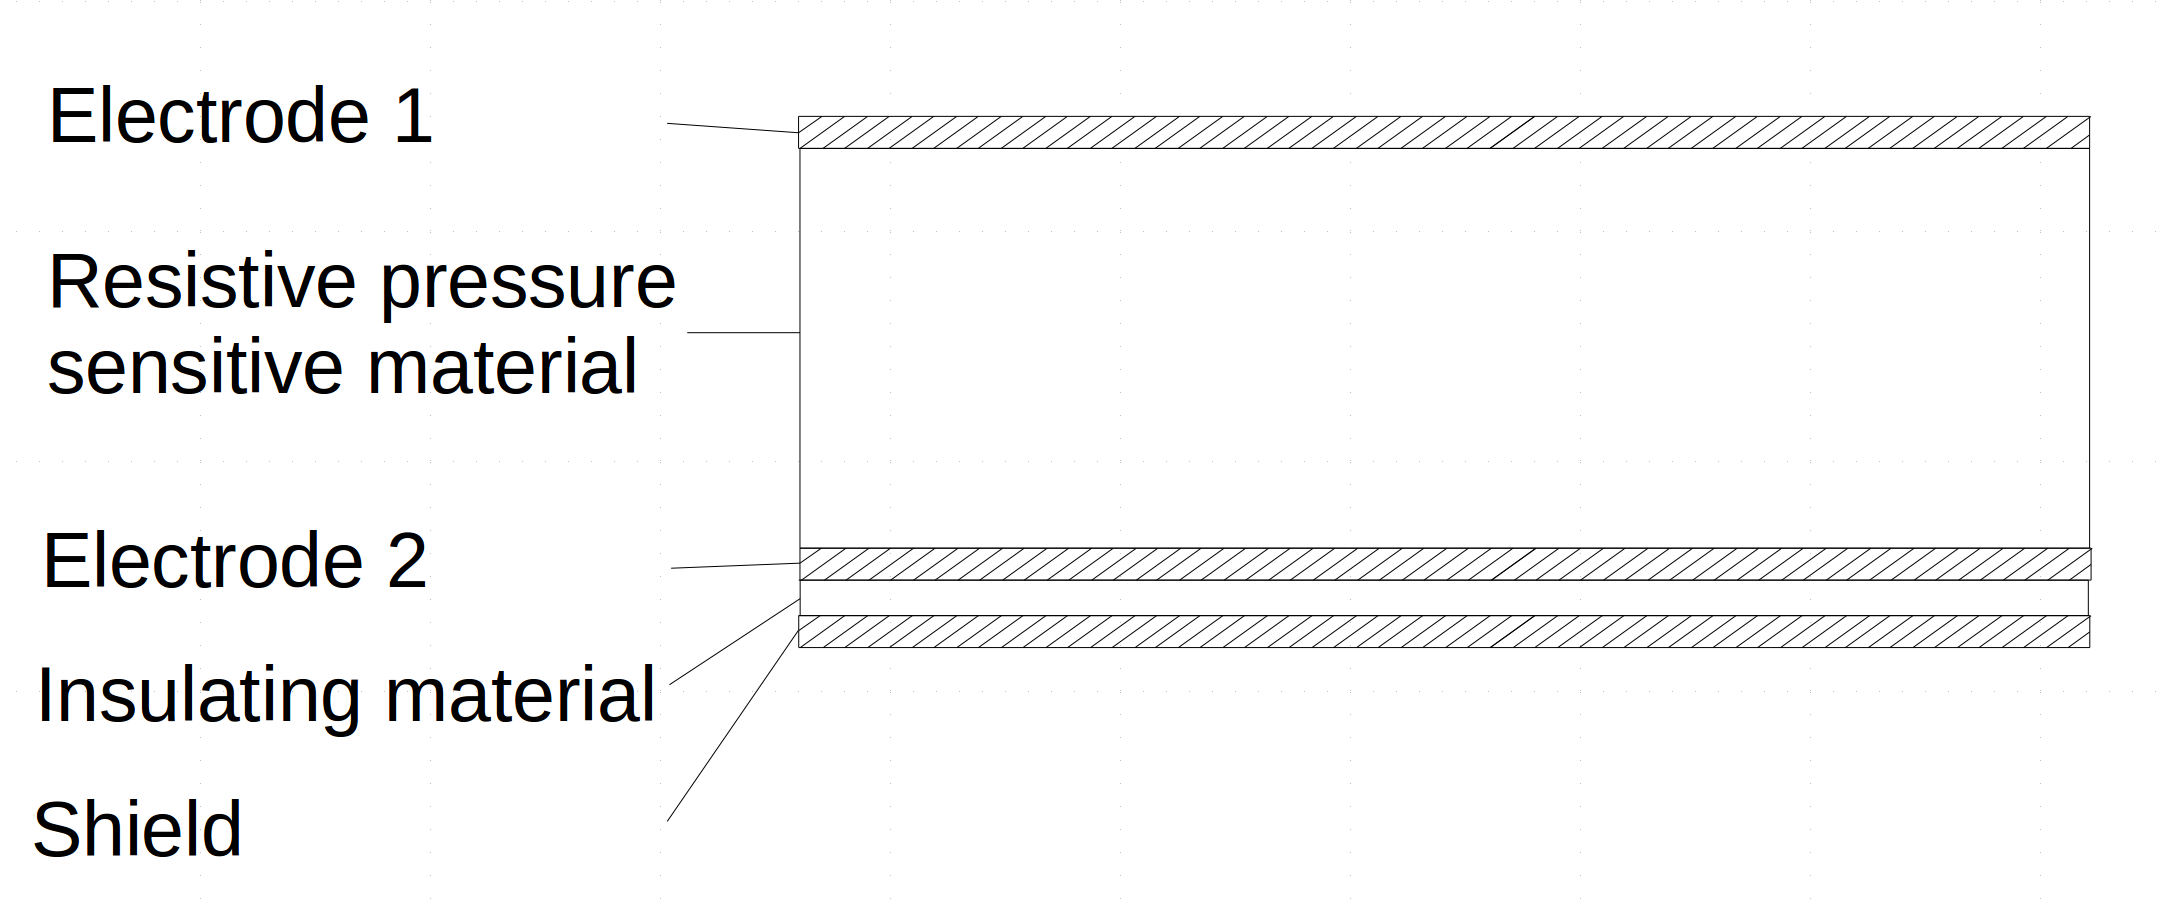
\includegraphics[width=0.9\columnwidth]{figures/stackup}
  \caption{Stackup for pressure and presence sensor with
shield}~\label{fig:stackup}
\end{figure}

\subsection{Relevancy}
It can be imagined that the PrePre could be integrated into garments, accessories, furniture, automotive and other places of human computer interaction.  The sensor is designed to the human body and the scale of the human hand.  The soft and flexible nature of the e-textile sensor allows for its implementation on a multitude of surfaces that the hand typically interacts with.  This includes clothing and accessories. 

\section{Technical Aspects}
\subsection{Resistive Pressure Sensors}
Low cost pressure sensors are often made by sandwiching flexible electrodes
with a layer of flexible moderately conductive material in between. The
moderately conductive material is usually made of a carbon impregnated polymer
with a specific structure that allows it to be squeezed together. The material
can be considered as having many parallel resistors. When the material is
compressed some of the resistors will be partially short-circuited due to
non-linear elastic deformations. The partial short-circuits result in a lower
overall resistance of the structure. This is visualized
in Figure \ref{fig:pressure_sensor}.



\subsection{Capacitive Touch / Distance Sensors}
Capacitive sensors are popular sensors in embedded computing due to their low cost
and capabilities of detecting approaching human body parts, which allows the
object to give feedback to the user even before the user is physically touching
the object. The physics behind sensors that measure self-capacitance is that one
plate of the capacitor is formed by the sensor and the other plate is formed by
nearby grounded objects such as humans. The capacitance is a function of area
and distance, as shown by the well-known parallel plate model

\begin{equation}
C = {{\varepsilon A} \over {d}}
\end{equation}

where $C$ is the capacitance, $\varepsilon$ is the permittivity of the material
between the plates (approximately $8.85418 \cdot 10^{-12} ~ \textrm{F/m}$ for
air), $A$ is the overlapping area of the plates and $d$ is the distance between
the plates.

% \begin{marginfigure}
% \begin{minipage}{\marginparwidth}
\begin{figure}
\centering
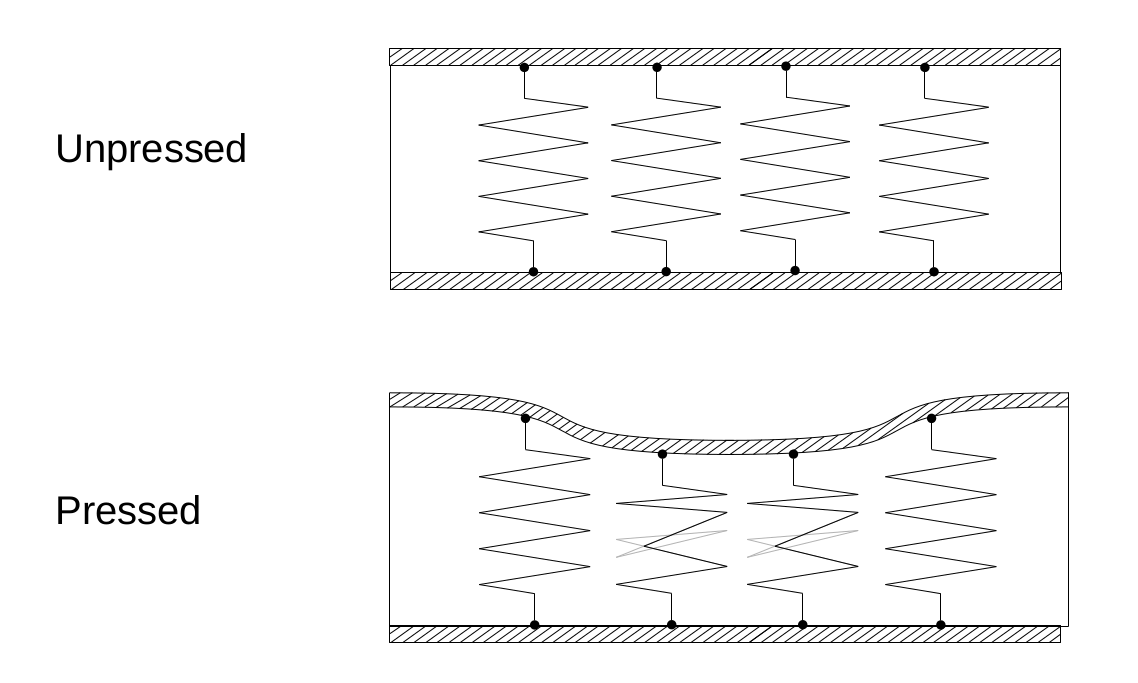
\includegraphics[width=0.9\columnwidth]{figures/resistive_sensor}
 \caption{Conceptual model of a pressure sensor. Compressing the sensor causes
  partial short-circuits which lowers the overall resistance of the
  structure.}~\label{fig:pressure_sensor}
\end{figure}
% \end{minipage}
% \end{marginfigure}


For many use cases of capacitive touch, the permittivity and area do not change
significantly and thus the capacitiance is a measure for the distance between
the sensor and the body part.

There are many different methods to measure
self-capacitance, two of those will be briefly discussed here.

\subsubsection{R-C Charge Method}
A very popular method in the Do It Yourself (DIY) community is the R-C charge
method. In this method the charge and discharge times of a resistor-capacitor
combination is measured. Since the resistor is fixed value, this is a measure
for the value of the capacitor. A detailed description can be found in FIXME:
ADD REFERENCE 

An intrinsic feature of capacitive touch sensors is that the
electric field needs to fringe out of the object to be able to sense the human
body and due to this fringing, the electric field is also easily disturbed by
other electric fields or nearby grounded objects such as 110 / 230 V wires,
electronic devices or metal structures. The slow measurement method of the R-C charge
method makes it more difficult to filter out these disturbances, leading to poor
performance of the sensor and poor experiences of capacitive touch for users of
the objects which use this method.



\subsubsection{CVD Method}
Another well-known method for self-capacitance does not rely on R-C charge times
but instead relies on charge distribution between the sample and hold capacitor
of an ADC ($\textrm{C}_{\textrm{S\&H}}$) and the capacitive sensor. This method
is called Capacitive Voltage Division (CVD).

\begin{marginfigure}
\begin{minipage}{\marginparwidth}
\centering
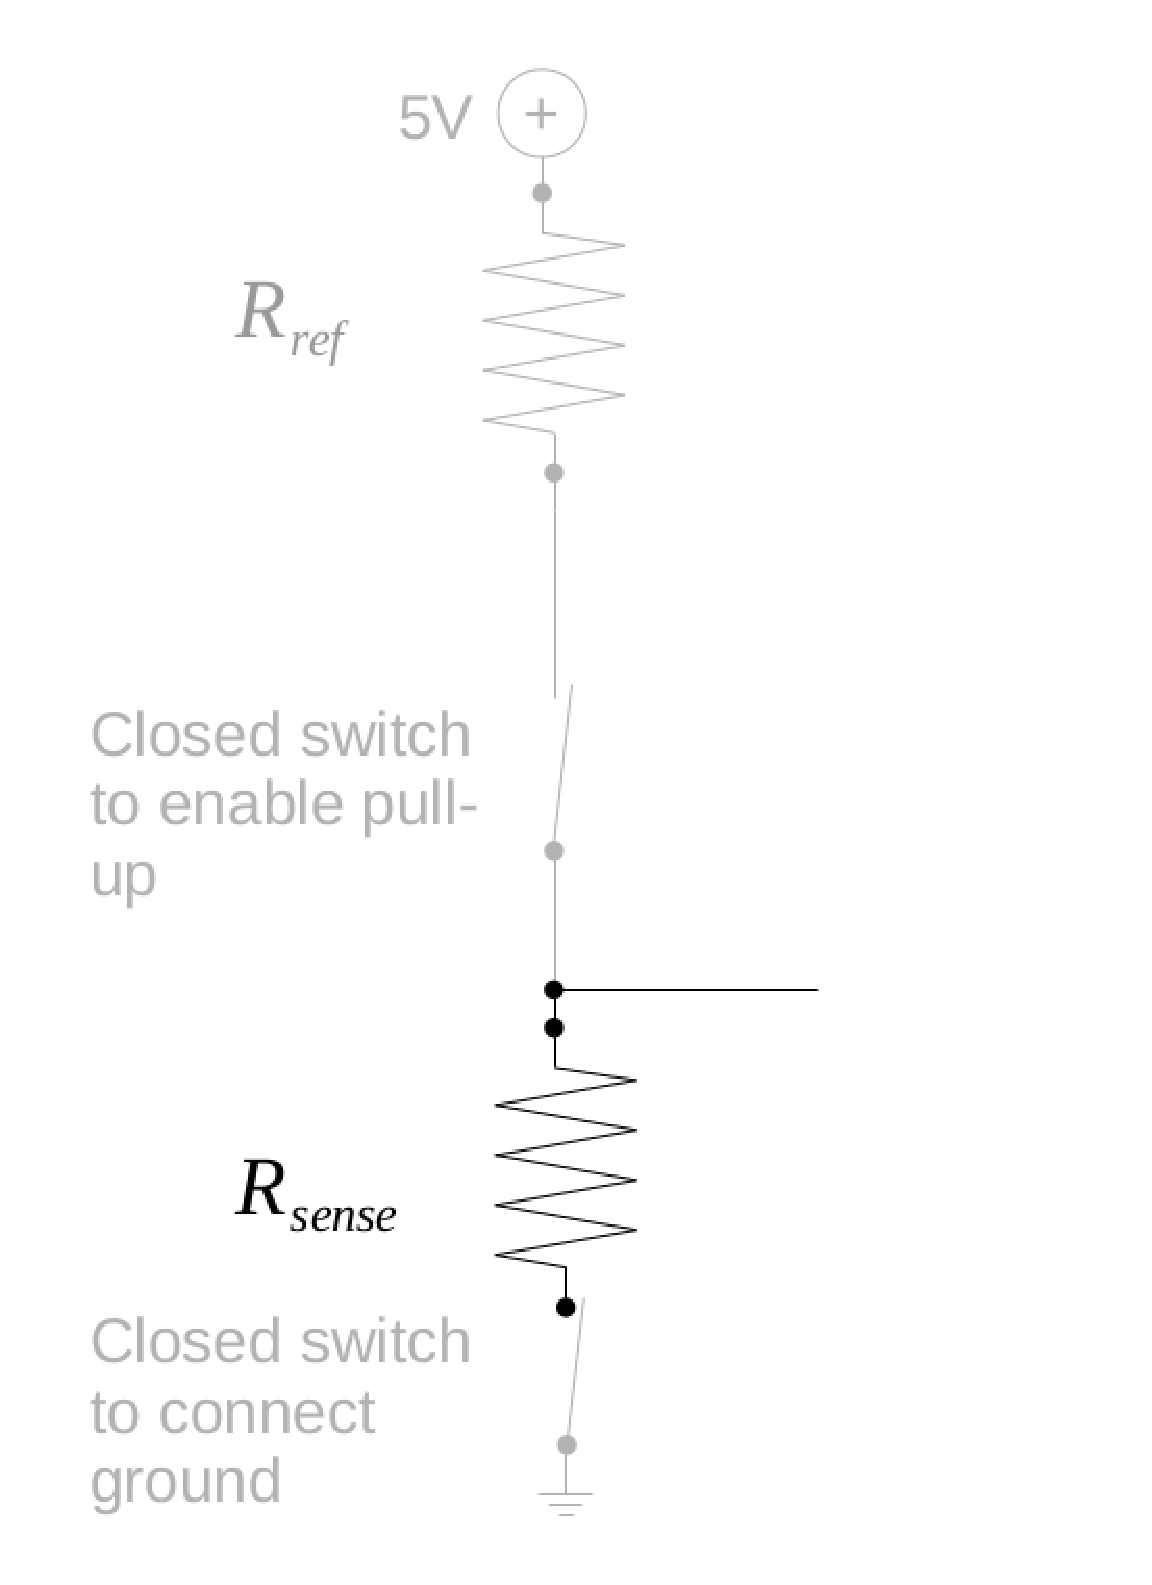
\includegraphics[width=0.9\columnwidth]{figures/cap_res_setup_res}
\caption{Resistive pressure sensor used in capacitive and resistive setup in
resistive sensing mode. Grey items are internal to the
microcontroller.}~\label{fig:cap_res_setup_res}
\end{minipage}
\end{marginfigure}

\begin{marginfigure}
\begin{minipage}{\marginparwidth}
\centering
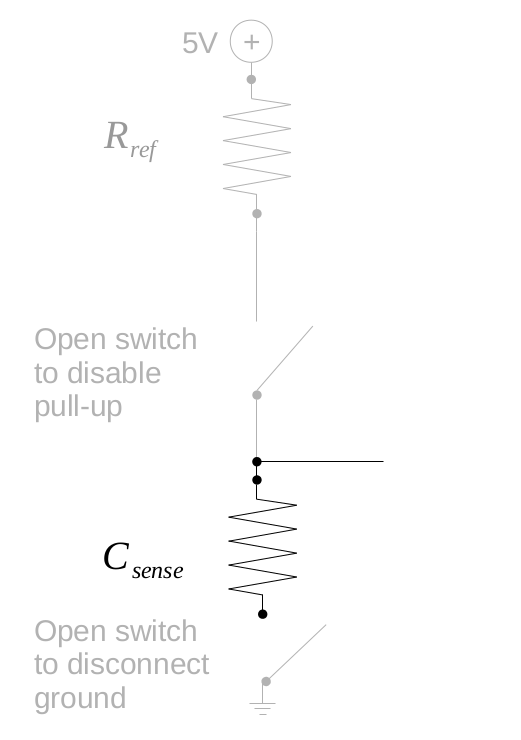
\includegraphics[width=0.9\columnwidth]{figures/cap_res_setup_cap}
\caption{Resistive pressure sensor used in capacitive and resistive setup in
capacitive sensing mode. Grey items are internal to the
microcontroller.}~\label{fig:cap_res_setup_cap}
\end{minipage}
\end{marginfigure}

In this method, no external resistor is required and the sensor plate is
directly connected to an analog input pin. The microcontroller starts a
measurement by configuring this pin as a digital output and making this output low,
thereby discharging the sensor. Next, the microcontroller connects the internal
ADC to its supply voltage, which charges $\textrm{C}_{\textrm{S\&H}}$ to a fixed
amount of charge which depends only on the capacitance
$\textrm{C}_{\textrm{S\&H}}$ and the supply voltage.

After the sensor pin is discharged and $\textrm{C}_{\textrm{S\&H}}$ is
charged, the sensor pin needs to be reconfigured as analog input and the
multiplexer of the ADC needs to be switched to this input. This will
redistribute the charge on $\textrm{C}_{\textrm{S\&H}}$ over both
$\textrm{C}_{\textrm{S\&H}}$ and the capacitance of the sensor. A larger sensor
capacitance will result in a lower voltage on the sensor and the last step of
this method is to measure this voltage using the usual ADC functions.

Since this method does not rely on R-C discharge times but uses the internal and
usually much faster and higher resolution ADC, more filtering can be applied to the signal to remove
disturbance of other nearby objects and electronic devices. This results in a
superior performance and a better user experience.

\subsection{Using Resistive Pressure Sensors as Capacitive Distance Sensors}
The CVD method connects the sensor directly to the analog input of a
microcontroller, similar to the resistive sensor setup. The resistive sensor can
now be used to also measure capacitance by connecting the other electrode of the
sensor to a GPIO pin instead of ground. This setup is shown in Figures
\ref{fig:cap_res_setup_res} and \ref{fig:cap_res_setup_cap}.

Figure \ref{fig:cap_res_setup_res} shows the setup in resistive sensing mode,
which is a standard resitive divider setup using an internal pull resistor
as reference resistor and a digital output pin as ground to complete the
circuit.

Figure \ref{fig:cap_res_setup_cap} shows the same circuit but with the GPIO pins
reconfigured for capacitive sensing. In this setup, the internal pull up
resistor is not used and the to electrode of the pressure sensor is only
connected to the analog input. The bottom electrode is connected to a pin that
is configured as digital input, which effectively means that the sensor is
floating. This is exactly the setup that is needed for the CVD method.

Since the ADC in modern microcontrollers is very fast (typically 1 million
samples per second or more), the microcontroller can rapidly switch between
resistive sensing and capacitive sensing modes and use the same sensor for both
resisitive pressure sensing and capacitive presence sensing.

\section{Software Features}
In many resistive pressure sensing or capacitive presence sensing
applications relative measurements are sufficient. In such cases, a state
machine which tracks any background variations on the signal level is a simple
and effective method to reduce noise. In our case, both the resistive sensor
signals and the capacitive sensor signals use the following state machine where
each signal has its own instance and its own parameter settings.

The state machine for each sensor can be in five states: Calibrating, Released,
Released to Pressed, Pressed and Pressed to Released.
This is shown in Figure \ref{fig:state_machine}.

In the Calibrating and Released states, the background variations are tracked
using an exponential decaying filter and stored in average $a$. In all other
states the background variations are not tracked. In the Released state, if the
most recent measurement $x$ is more than $P$ counts below average $a$, the state
is changed to Released to Pressed. If in the next measurement $x$ is less
than $P$ counts below the average, the state is changed back to Released. If
however the next $C$ measurements are all more than $P$ counts below this
average, the state is changed to Pressed.

% \begin{marginfigure}
% \begin{minipage}{\marginparwidth}
\begin{figure}
\centering
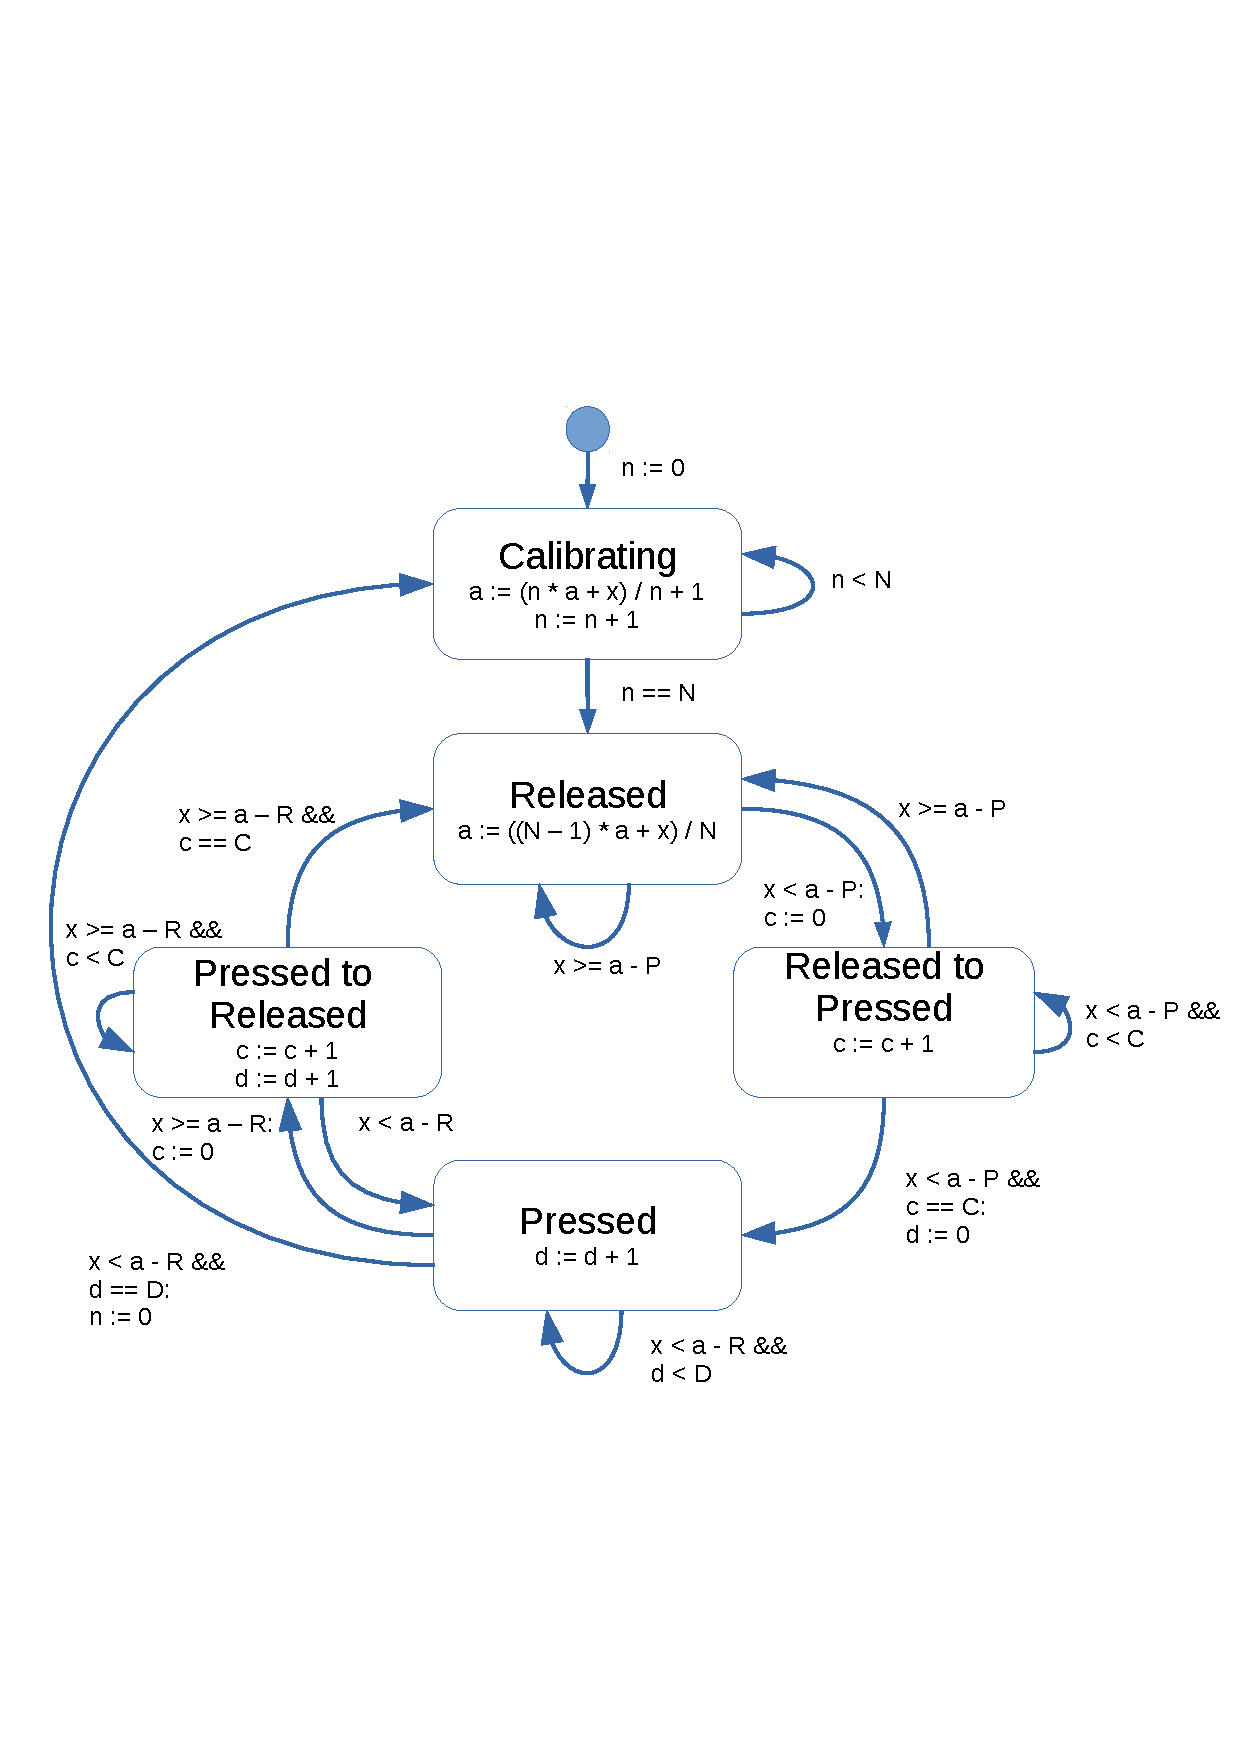
\includegraphics[trim={0 6.2cm 0 6.8cm},clip,width=0.9\columnwidth]{figures/state_machine}
 \caption{State machine for resistive and capacitive measurements to track
background variations.}~\label{fig:state_machine}
\end{figure}
% \end{minipage}
% \end{marginfigure}

Similarly the state moves from the Pressed state to the Pressed to Released
state and from Pressed to Released to the Released state.

To account for stuck buttons (for example: when the user unintentionally placed
a large conductive object very close to the capacitive touch sensor while the
sensor was in Released state), there is a maximum time that the sensor can be in
the Pressed state. If after this time the sensor is still in the Pressed state,
it is changed to the Calibrating state and the sensor will start recalibrating.

By changing the parameters $N$, $C$, $P$ and $R$ the amount of filtering and
speed of detection can be tuned to the application. Once they are tuned
properly, the difference of $x$ and $a$ is a measure for how close a user is to
the sensor (in capacitive sensing mode) or for how much pressure a user applies
to the sensor (in resistive sensing mode).

%FIXME: ADD REFERENCE TO STATE MACHINE 

\section{Shielding}
In capacitive sensing mode, the sensor is also sensitive on the underside. If
the distance between the underside of the sensor and the human body is
relatively constant, tuning of the state machine could be sufficient to filter
this out and make the sensor only sensitive to large and / or rapid variations.

However, some applications such as lose fitting clothing require more filtering
and benefit from a shield underneath the
sensor. Connecting this shield to ground effectively removes all of the
capacitance variation but also reduces the sensitivity of the sensor. By
connecting the sensor itself to the input of a 1 x opamp and the output of the
opamp to the shield, the voltage of the shield is always very close to the
voltage on the sensor itself. As a result, the electric field underneath the
sensor is virtually zero and no sensitivity is lost. Note that for proper
shielding, also the cable to the sensor should be shielded. A schematic diagram
of this setup is shown in Figure \ref{fig:shield_circuit}.

%FIXME: ADD REFERENCE TO SHIELDING

% \begin{marginfigure}
% \begin{minipage}{\marginparwidth}
\begin{figure}
\centering
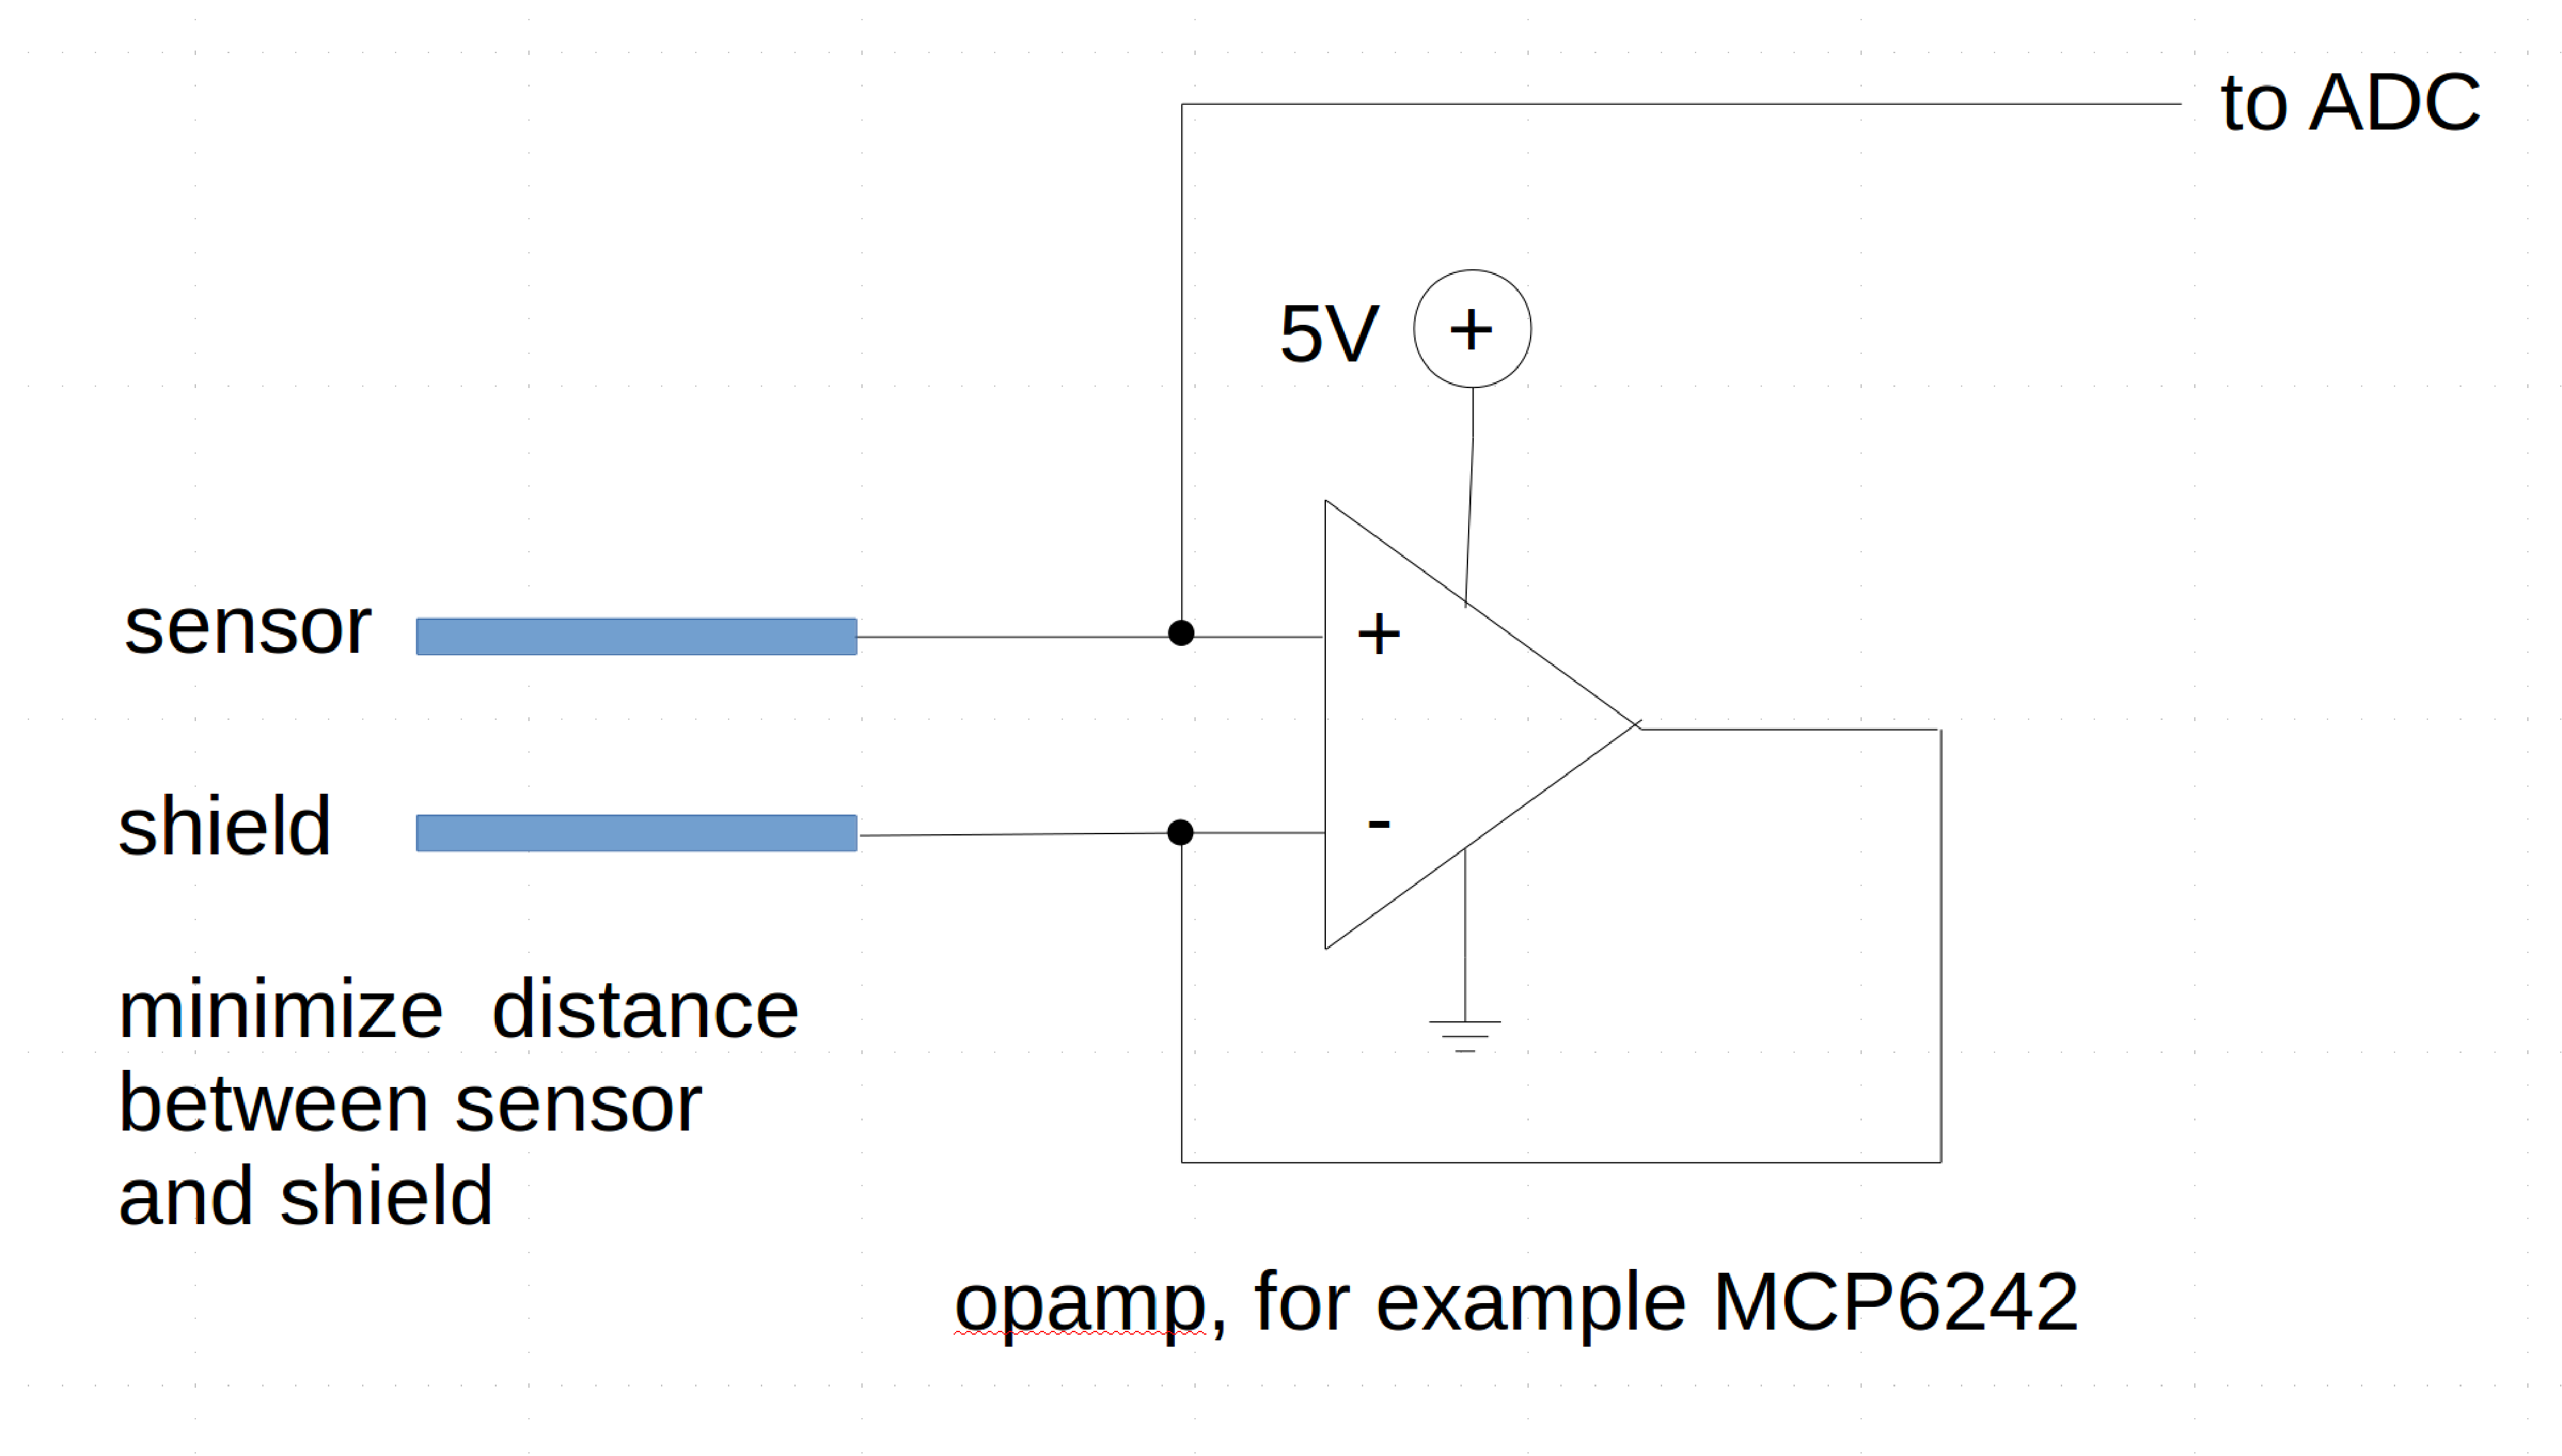
\includegraphics[width=0.9\columnwidth]{figures/shield_circuit}
  \caption{Circuit to shield underside of capacitive
sensor.}~\label{fig:shield_circuit}
\end{figure}
% \end{minipage}
% \end{marginfigure}

% \section{Mechanical Features}
% An overview of the stackup of the total sensor is shown in Figure
% \ref{fig:stackup}. In this figure, the electrode and shield material can be
% conductive textile, the insulating material can be any non-compressable
% insulating material (for example cotton) and the pressure sensitive material can
% be Velostat or ESD foam.


\section{Conclusion}
The possibilities of a reliable, textile, soft presence and pressure sensor are numerous.  This reliability was detailed in the combination of capacitive distance sensing using the CVD method for presence sensing with resistive sensing for pressure
sensing. The robustness of the CVD method as well as the required circuit and
microcontroller features make it ideal to combine with existing resistive pressure sensing applications to enhance the user experience by not only sensing how hard a user presses on a button but already giving feedback to the user when approaching the button. The choice of textiles increases the reliability and performance of the sensor in their specific contexts. In the use of a shoes we can understand not only how hard the foot is being pressed, but if the foot is disconnecting from the shoe.  In garments we can understand how multiple people approach and touch each other in performance or everyday activities. In the context of a automative steering wheel we can understand not only where someone is touching, but how they move there hands when engaged in an maneuver such as turning a corner.
The use of multiple sensors for greater movement vector and specific specific touch location sensing is a serious possibility that the authors intend to explore further.  
\section{Acknowledgements}
The authors would like to thank the Wearable Senses Lab, /dSearch Lab and E-Labs along with the Designing Quality in Interaction group of the Industrial Design department of the Eindhoven University of Technology. Support for this project also comes from the Marie Curie Horizon 2020 Action ArcInTexETN. Special thanks to Dr. Oscar Tomico and Dr. Stephan Wensveen of TU Eindhoven.
% BALANCE COLUMNS
\balance{} 
% REFERENCES FORMAT
% References must be the same font size as other body text.
\bibliographystyle{SIGCHI-Reference-Format}
\bibliography{sample}

\end{document}

%%% Local Variables:
%%% mode: latex
%%% TeX-master: t
%%% End:
